\documentclass[11pt]{amsart}
\usepackage{enumitem}
\usepackage{setspace}
\onehalfspacing
\usepackage{geometry}                % See geometry.pdf to learn the layout options. There are lots.
\geometry{letterpaper}                   % ... or a4paper or a5paper or ... 
%\geometry{landscape}                % Activate for for rotated page geometry
%\usepackage[parfill]{parskip}    % Activate to begin paragraphs with an empty line rather than an indent
\usepackage{graphicx}
\usepackage{amssymb}
\usepackage{amsmath}
\usepackage{epstopdf}
\usepackage[linesnumbered,vlined,algoruled]{algorithm2e}
\usepackage{url}
\usepackage{mathtools}
\DeclarePairedDelimiter{\ceil}{\lceil}{\rceil}
\DeclarePairedDelimiter{\floor}{\lfloor}{\rfloor}
\DeclareGraphicsRule{.tif}{png}{.png}{`convert #1 `dirname #1`/`basename #1 .tif`.png}
\DeclareMathOperator*{\argmax}{arg\,max}
\DeclareMathOperator{\argmin}{arg\,min}
\setlength{\parskip}{0.5 em}

\title{Computing Extremely Accurate Quantiles Using $t$-Digests}
\author{Ted Dunning}
\address{Ted Dunning \\ MapR Technologies, Inc \\ San Jose, CA}
\email{ted.dunning@gmail.com}
\author{Otmar Ertl}
\email{otmar.ertl@gmail.com}
\date{}                                           % Activate to display a given date or no date
\begin{document}
\begin{abstract}
Two variants of an on-line algorithm for computing approximations of rank-based statistics are presented that allow controllable accuracy, particularly near the tails of the distribution.  Moreover, this new algorithm can be used to compute hybrid statistics such as trimmed means in addition to computing arbitrary quantiles.  An unusual property of the method is that it allows a quantile $q$ to be computed with an accuracy relative to $q\,( 1-q)$ rather than with an absolute accuracy as with most methods.  This new algorithm is robust with respect to highly skewed distributions or highly ordered datasets and allows separately computed summaries to be combined with no loss in accuracy.

An open-source Java implementation of this algorithm is available from the author. Implementations in Go and Python are also available.
\end{abstract}
\maketitle
\section{Introduction}
Given a set of numbers, it is often desirable to compute rank-based statistics such as the median, 95-th percentile or trimmed means in an on-line fashion. In many cases, there is an additional requirement that only a small data structure needs to be kept in memory as data is processed in a streaming fashion.  Traditionally, such statistics have been computed by sorting the data and then either finding the quantile of interest by interpolation or by re-processing all samples within particular quantile ranges.  This sorting approach can be infeasible for very large datasets or when quantiles of many subsets must be calculated. This infeasibility has led to interest in on-line approximate algorithms. Previous algorithms can compute approximate values of quantiles using constant or only weakly increasing memory footprint, but these previous algorithms cannot provide constant relative accuracy.  The new algorithm described here, the $t$-digest, provides constant memory bounds and constant relative accuracy while operating in a strictly on-line fashion.

\subsection{Previous work}

One early algorithm for computing on-line quantiles is described by Chen, Lambert and Pinheiro in \cite{Chen2000}.  In that work specific quantiles were computed by incrementing or decrementing an estimate by a value proportional to the simultaneously estimated probability density at the desired quantile.  This method is plagued by a circularity in that estimating density is only possible by estimating yet more quantiles.  Moreover, this work did not allow the computation of hybrid quantities such as trimmed means.

Munro and Paterson\cite{munro1980} provided an alternative algorithm to get a precise estimate of the median.  This is done by keeping $s$ samples from the $N$ samples seen so far where $s << N$ by the time the entire data set has been seen.  If the data are presented in random order and if $s = \theta(N^{1/2} \log N)$, then Munro and Paterson's algorithm has a high probability of being able to retain a set of samples that contains the median.  This algorithm can be adapted to find a number of pre-specified quantiles at the same time at proportional cost in memory.  The memory consumption of Munro-Paterson algorithm is, however, excessive if precise results are desired.  Approximate results can be had with less memory, however.  

A more subtle problem is that the implementation of Munro and Paterson's algorithm in Sawzall\cite{sawzall} and the Datafu library\cite{datafu} uses a number of buckets computed from the GCD of the desired quantiles.  This means that if you want to compute the $99$-th, $99.9$-th and $99.99$-th percentiles, a thousand buckets are required, each of which requires the retention of many samples. We will refer to this implementation of Munro and Paterson's algorithm as MP01 in results presented here.

One of the most important results of the work by Munro and Paterson was a proof that computing any particular quantile exactly in $p$ passes through the data requires $\Omega(N^{1/p})$ memory. For the on-line case, $p=1$, which implies that on-line algorithms cannot guarantee to produce the precise value of any particular quantile. This result together with the importance of the on-line case drove subsequent work to focus on algorithms to produce approximate values of quantiles.

Greenwald and Khanna\cite{Greenwald-space-efficient-online-quantiles} provided just such an approximation algorithm that is able to provide estimates of quantiles with controllable accuracy. This algorithm (which we shall refer to as GK01 subsequently in this paper) requires less memory than Munro and Paterson's algorithm and provides approximate values for pre-specified quantiles.

An alternative approach is described by Shrivastava and others in \cite{qdigest}.  In this work, incoming values are assumed to be integers of fixed size. Such integers can trivially be arranged in a perfectly balanced binary tree where the leaves correspond to the integers and the interior nodes correspond to bit-wise prefixes. This tree forms the basis of the data structure known as a Q-digest.  The idea behind a Q-digest is that in the uncompressed case, counts for various values are assigned to leaves of the tree.  To compress this tree, sub-trees are collapsed and counts from the leaves are aggregated into a single node representing the sub-tree such that the maximum count for any collapsed sub-tree is less than a threshold that is a small fraction of the total number of integers seen so far.  Any quantile can be computed by traversing the tree in left prefix order, adding up counts until the desired fraction of the total is reached.  At that point, the count for the last sub-tree traversed can be used to interpolate to the desired quantile within a small and controllable error.  The error is bounded because the count for each collapsed sub-tree is bounded.

The salient virtues of the Q-digest are
\begin{itemize}[nosep, topsep=-10pt]
\item the space required is bounded proportional to a compression factor $k$
\item the maximum error of any quantile estimate is proportional to $1/k$ and
\item the desired quantiles do not have to be specified in advance.
\vspace{10pt}
\end{itemize}

On the other hand, two problems with the Q-digest are that it depends on the set of possible values being known in advance and produces quantile estimates with constant error in $q$. In practice, this limits application of the Q-digest to samples which can be identified with the integers. Adapting the Q-digest to use an balanced tree over arbitrary elements of an ordered set is difficult.  This difficulty arises because rebalancing the tree involves sub-tree rotations and these rotations may require reapportionment of previously collapsed counts in complex ways.  This reapportionment could have substantial effects on the accuracy of the algorithm and in any case make the implementation much more complex because the concerns of counting cannot be separated from the concerns of maintaining a balanced tree.  
\subsection{New contributions}
The work described here introduces a new data structure known as the $t$-digest. The $t$-digest differs from previous structures designed for computing approximate quantiles in several important respects. First, although data is binned and summarized in the $t$-digest, the range of data included in different bins may overlap. Second, the bins are summarized by a centroid value and an accumulated weight representing the number of samples contributing to a bin. Third, the samples are accumulated in such a way that only a few samples contribute to bins corresponding to extreme quantiles so that relative error is bounded instead of maintaining constant absolute error as with previous methods.

With the $t$-digest, accuracy for estimating the $q$ quantile is constant relative to $q(1-q)$.  This is in contrast to earlier algorithms which had errors independent of $q$.  The relative error bound of the $t$-digest is convenient when computing quantiles for $q$ near $0$ or $1$ as is commonly required.  As with the Q-digest algorithm, the accuracy/size trade-off for the $t$-digest can be controlled by setting a single compression parameter $\delta$ with the amount of memory required proportional only to $\Theta(\delta)$. 
\section{The $t$-digest}
A $t$-digest represents the empirical distribution of a set of numbers by retaining centroids of sub-sets of numbers. Algorithmically, there are two important ways to form a $t$-digest from a set of numbers. One version keeps a buffer of incoming samples. Periodically, this buffer is sorted and merged with the centroids computed from previous samples. This merging form of the $t$-digest algorithm has the virtue of allowing all memory structures to be allocated statically. On an amortized basis, this buffer-and-merge algorithm can be very fast especially if the input buffer is large. The other major $t$-digest algorithm is more akin to a clustering algorithm in which new samples are selectively added to the nearest centroid.  Both algorithms are described here and implementations for both widely are available. 

\subsection{The basic concept}
Suppose first, for argument's sake, that all of the samples $X=x_1 \ldots x_n$ are presented in ascending order. Since the samples are ordered, we can use interpolation on the indexes of each sample to determine the value of the empirical quantile for any new value. 

A $t$-digest is formed from the sequence of points by grouping all of the samples into sub-sequences of samples, $X = \lbrace s_1 | s_2 | \ldots | s_m \rbrace$ where $s_i = \lbrace x_{\mathtt {left}(i)} \ldots x_{\mathtt{right}(i)} \rbrace$.  The beginning and end of each sub-sequence is chosen so that the sub-sequence is small enough to get accurate quantile estimates by interpolation, but large enough so that we don't wind up with too many sub-sequences. Importantly, we force sub-sequences near the ends to be small while allowing sub-sequences in middle to be larger in order to get fairly constant relative accuracy.

To limit the sub-sequence size in this way, we define a mapping from quantile $q$ to a notional index $k$ with compression parameter $\delta$. This mapping is known as the scaling function and a preferred choice of function for the $t$-digest is 
\[
k(q, \delta) = \delta \left( {\frac {\sin^{-1} (2q-1)} \pi}   + {1 \over 2} \right)
\]
The mapping $k$ is monotonic with minimum value  $k(0)=0$ and maximum value  $k(1)=\delta$.  Figure \ref{fig:k-q-plot} shows the relationship between $k$ and $q$ for $\delta=10$. In this figure, the horizontal lines are spaced uniformly at integer values of $k$ which puts the corresponding vertical lines much closer together near $q=0$ and $q=1$.

Next we require that the $k$-size of each sub-sequence be less than $1$,
\[
K(i) = k \left (\mathtt{right}(i)/n \right) - k \left ((\mathtt{left}(i)-1)/n \right) \le 1
\]
and that adjacent sub-sequences cannot be merged by forcing
\[
K(i) + K(i+1) > 1
\]
for all $i=1\ldots m-1$. These conditions imply that the mean value of $K(i)$ is in $(1/2, 1]$ which means that the number $m$ of such maximally merged groups is bounded according to $ \lfloor\delta\rfloor \le m < 2\left \lceil\delta \right \rceil$. 

\begin{figure}[htbp] %  figure placement: here, top, bottom, or page
   \centering
   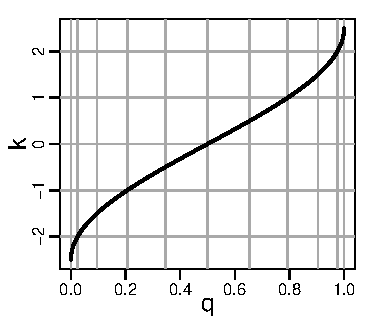
\includegraphics[width=2.3in]{k-q-plot.pdf} 
   \caption{The scaling function translates the quantile $q$ to the scaling factor $k$ in order to give variable size steps in $q$. Limiting sizes in terms of maximum values of $k$ allows better accuracy near $q=0$ or $q=1$ because bins near there will be smaller. The scaling function is carefully chosen to adjust bin sizes for best relative accuracy. Conventional quantile algorithms can be viewed as using a linear scaling function which results in bin sizes that are constant with respect to $q$.}
   \label{fig:k-q-plot}
\end{figure}
The introduction of the concept of a scaling function provides a useful way to see the core distinction between conventional percentile approximation algorithms that use equal-sized bins and the $t$-digest with its non-equal bin sizes. The only really necessary characteristics of a scaling function is that be monotonic and satisfy the constraints that $k(0)=0$ and $k(1)=\delta$. The linear function $k(q) = \delta q$ clearly meets these requirements and thus would be an acceptable scaling function. Using a linear scaling function results in uniform bin sizes and constant absolute error just as in previously reported quantile approximation algorithms. The $t$-digest, in contrast, has a non-linear scaling function which was chosen to give non-equal bin sizes and constant relative accuracy.

Once we have formed a $t$-digest by binning the original sequence into sub-sequences that satisfy the size limit, we can estimate quantiles using interpolation between the end-points of each bin. This is similar to what is done in other quantile estimation algorithms such as Greenwald-Khanna and will give errors that scale roughly quadratically in the number of samples in each sub-sequence. The $t$-digest, having smaller number of samples in bins near $q=0$ or $q=1$ will obviously have better accuracy there. The only wrinkle is that with a $t$-digest contains the centroids of the samples in a bin instead of the end-points. Estimating quantiles requires that the boundaries of the bins be estimated first and then used to interpolate as before. 

In general, there are many partitions of $X$ that valid result in a $t$-digest. As long as the result is subject to the size contraint, however, any such $t$-digest will perform similarly in terms of accuracy.

Figure \ref{fig:linear-interpolation} shows an example of how error bounds are improved by the strategy of keeping bins small near extreme values of $q$. 

\begin{figure}[h] %  figure placement: here, top, bottom, or page
   \centering
   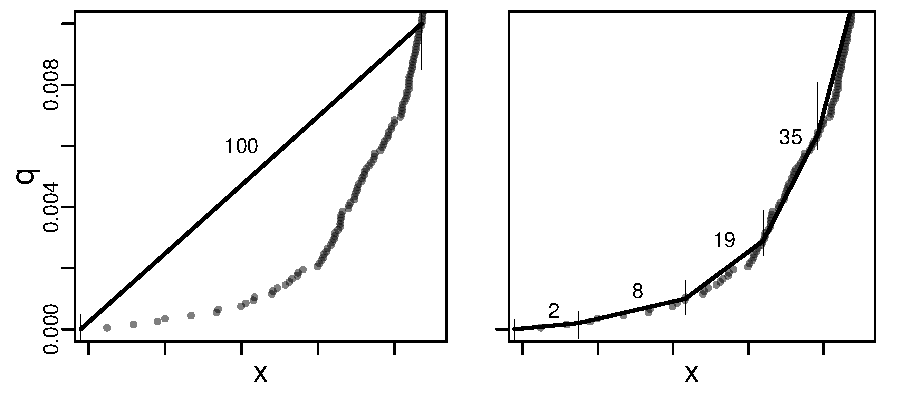
\includegraphics[height=2.in, clip]{linear-interpolation.pdf} 
   \caption{The left panel shows linear interpolation of a cumulative distribution function near $q=0$ with $100$ equal sized bins applied to $10,000$ data points sampled from an exponential distribution. The right panel shows the same interpolation with variable size bins as given by a $t$-digest with $\delta=100$. The numbers above the data points represent the number of points in each bin. }
   \label{fig:linear-interpolation}
\end{figure}
This figure shows roughly the first percentile of $10,000$ data points sampled using $x \sim \log u$ where $u \sim \mathrm{Uniform}(0,1)$. In the left panel, the data points have been divided into 100 bins, each with 100 data points, of which only the left-most bin is visible. The use of equal sized bins means that the interpolated value of $q$ in the left panel of the figure has a substantial and unavoidable error. The right panel, on the other hand, shows a $t$-digest with roughly the same number of bins ($102$ instead of $100$), but with many fewer points in bins near the $q=0$. A value of $\delta=100$ is used here which is quite typical in practical use. 

Of course, since we have to put every sample into some bin, filling some bins with fewer than $100$ samples requires that other bins must have more than $100$ samples or we have to have more bins. Importantly, having fewer samples in the bins near the ends improves accuracy substantially, but increasing the bin sizes near $q=1/2$ has a much weaker effect on accuracy. In this particular example, the first bin has only 2 samples and thus zero error and the second bin has only 10 samples giving 100 times smaller error while the central bins in the $t$-digest have about $1.6$ times more samples than the uniform case, increasing errors by about two and a half times relative to equal sized bins. The overall effect is that quantile estimation accuracy is dramatically improved at the extremes but only modestly impaired in the middle of the distribution.
\subsection{Merging independent $t$-digests}
In the previous section, the algorithm for forming a $t$-digest took a set of unweighted points as inputs. Nothing, however, would prevent the algorithm from being applied to a set of weighted points. As long as individual weights are smaller than the size limit imposed by the scaling function, the result will still be a well-formed $t$-digest.

If we form independent $t$-digests $t_x$ and $t_y$ from separate sequences $X$ and $Y$, these $t$-digests can clearly be used to estimate quantiles of $X \cup Y$ by separately computing quantiles for $X$ and $Y$ and combining the results. More usefully, we can form a new $t$-digest by taking the union of the centroids from $t_x$ and $t_y$ and merging the centroids whenever they meet the size criterion. The resulting $t$-digest will not be the same as if we had computed a $t$-digest $t_{X \cup Y}$ from all of the original data at once even though it will meet the same size constraint. In practice, perhaps surprisingly, a merged $t$-digest gives accuracy comparable to what we would get from $t_{X\cup Y}$.

The observation that $t$-digests formed by merging other digests will produce accurate quantile estimates has substantial empirical support, even with highly structured data sets such as ordered data or data with large numbers of repeated values, but there is, as yet, no rigorous proof of any accuracy guarantees. The size bounds are, nevertheless, are well established.

The ability to merge $t$-digests makes parallel processing of large data-sets relatively simple since independent $t$-digests can be formed from disjoint partitions of the input data and then combined to get a $t$-digest representing the complete data-set.

A similar divide and conquer strategy can be used to allow $t$-digests to be used in OLAP systems. The idea is that queries involving quantiles of subsets of data can be approximated quickly by breaking the input data set into subsets corresponding to each unique combination of selection factors. A single $t$-digest is then pre-computed for each unique combination of selection factors. To the extent that all interesting queries can be satisfied by disjoint unions of such primitive subsets, the corresponding $t$-digests can be combined to compute the desired result.

\subsection{Progressive merging algorithm}
The observation that merging $t$-digests gives good accuracy suggests a practical algorithm for constructing a $t$-digest from a large amount of data. The basic idea is to collect data in a buffer. When the buffer fills, or when a final result is required, sort the buffer and the existing centroids together, and pass through the combined set of points and centroids, merging points or centroids together whenever the size limits can be satisfied by the merged value. With an arbitrarily large buffer, this algorithm reduces to the original approach for constructing a $t$-digest from sorted data since the overall effect is simply a single merging pass through all the data. For smaller buffer sizes, however, many merge passes are required to process a large amount of data. This is essentially equivalent to forming independent $t$-digests on buffers of data and then sequentially merging them to get the final result.

The operation of merging a buffer's worth of samples into an existing set of centroids is shown in Algorithm \ref{alg:merge}. Note that the check on the size bound is optimized to only require only as many evaluations of $k(q)$ during the merge as there are output values in $C'$. This is done by computing the bounding value $q_{limit} = k^{-1}(k(q, \delta) + 1, \delta)$ each time a new centroid is emitted. This allows the conditional to be triggered based on comparisons of $q$ so that if many points are merged, no additional calls to $k$ are needed. If $n \gg 2 \left \lceil \delta \right \rceil$, this can result in a considerable speedup since computing $\sin^{-1}$ is expensive. Note also that this algorithm allows static allocation of all data structures as four arrays of primitive values, avoiding any dynamic allocation or structure boxing/unboxing.
\begin{algorithm}[ht]
\SetKw{KwTo}{in}\SetKwFor{For}{for}{\string:}{}
\SetKwIF{If}{ElseIf}{Else}{if}{:}{elif}{else:}{}
\SetKwFor{While}{while}{:}{fintq}
\SetKwFor{For}{for}{\string:}{}
 \label{alg:merge}
\SetNoFillComment
\KwIn{Sequence $C = [c_1 \ldots c_m]$ a $t$-digest containing real-valued, weighted centroids with components $\mathtt{sum}$ and $\mathtt{count}$ arranged in ascending order by mean, data buffer  $X = { x_1,\ldots x_n}$ of real-valued, weighted points, and compression factor $\delta$}
\KwOut{New ordered set $C'$ of weighted centroids forming a $t$-digest} 
$X \gets \mathtt{sort}(C | X)$\;
$ S = \sum_i x_i.\mathtt{count}$\;
$C' = \lbrack \, \rbrack, q_0 = 0$\;
$q_{limit}=k^{-1}(k(q_0, \delta)+1, \delta)$\;
$\sigma = x_1$\;
\For{$i \in 2\ldots(m+n)$} {
  $q = q_0 + (\sigma.\mathtt{count} + x_i.\mathtt{count})/S$\;
  \If {$q \le q_{limit}$} {
      $\sigma \gets \sigma + x_i$\;
  } \Else {
      $\mathtt{C'.append}(\sigma)$\;
      $q_0 \gets q_0 + \sigma.\mathtt{count}/S$\;
      $q_{limit} \gets k^{-1}(k(q_0, \delta)+1, \delta)$\;
      $\sigma \gets x_i$\;
  }
} 
$C'\mathtt{.append}(\sigma)$\;
\Return $ C' $\\
\caption{Merging new data into a $t$-digest}
\end{algorithm}

The run-time cost of the merge variant of the $t$-digest is a mixture of the frequent buffer inserts  and the rare periodic merges. The buffer inserts are very fast since they consist of an array write, index increment and an overflow test. The merges consist of the buffer sort and the merge itself. The merge involves a scan through both the buffer and the existing centroids plus a number of calls to $\sin^{-1}$ roughly equal to the size of the result and thus bounded by $2 \lceil \delta \rceil$. If $k_1$ is the input buffer size, the dominant costs are the sort and the $\sin^{-1}$ calls so the amortized cost per input value is roughly $C_1 \log k_1 + C_2 \lceil \delta \rceil / k_1$ where $C_1$ and $C_2$ are parameters representing the sort and $\sin^{-1}$ costs respectively. This overall amortized cost has a minimum where $k_1 \approx \delta\, C_2  / C_1$. The constant of proportionality should be determined by experiment, but micro-benchmarks indicate that $C_2 / C_1$ is in the range from $5$ to $20$ for a single core of an Intel i7 processor. In micro-benchmarks, increasing the buffer size to $10 \lceil \delta \rceil$ dramatically improves the average speed but further buffer size increases have much less effect.

\subsection{The clustering variant}

% boundary 

The basic outline of the clustering algorithm for constructing a $t$-digest is quite simple.  An initially empty ordered list of centroids, $C = [ c_1 \ldots c_m ]$ is kept.  Each centroid consists of a mean and a count.  To add a new value $x_n$ with a weight $w_n$, the set of centroids is found that have minimum distance to $x_n$.  This set is reduced by retaining only centroids with a count less than $4\delta q (1-q) n $ where $\delta$ controls the accuracy of quantile estimates and $q$ is the estimated quantile for the mean of the centroid.  If more than one centroid remains, one is selected at random.  If a centroid is found, then $(x_n,w_n)$ is added to that centroid.  It may happen that the weight $w_n$ is larger than can be added to the selected centroid.  If so, as much weight as possible is allocated to the selected centroid and the selection is repeated with the remaining weight.  If no satisfactory centroid is found or if there is additional weight to be added after all centroids with minimum distance are considered, then $x_n$ is used to form a new centroid and the next point is considered.  This procedure is shown more formally as Algorithm \ref{alg:full}.
 \begin{algorithm}[tb]
\SetKw{KwTo}{in}\SetKwFor{For}{for}{\string:}{}
\SetKwIF{If}{ElseIf}{Else}{if}{:}{elif}{else:}{}
\SetKwFor{While}{while}{:}{fintq}
\SetKwFor{For}{for}{\string:}{}
 \label{alg:full}
\SetNoFillComment
\KwIn{Ordered set of weighted centroids $C = \lbrace \rbrace$, sequence of real-valued, weighted points $X = \lbrace (x_1, w_1),\ldots (x_N, w_N)\rbrace$, and accuracy tolerance $\delta$}
\KwOut{final set $C=[c_1 \ldots c_m]$ of weighted centroids} 
\For{$(x_n, w_n) \in X$} {
  $z = \min | c_i.\mathtt{mean} - x |$\;
  $S = \lbrace c_i  :  |c_i.\mathtt{mean} - x| = z \wedge c_i.\mathtt{count} + w_n \le 4n\delta q(c_i) (1-q(c_i)) \rbrace $\;
   \While {$S \ne \lbrace \rbrace\wedge w_n > 0$} {
       Sample $c_j \sim \mathrm{Uniform}( S)$\;
       $\Delta w = \min(4n\delta q(c_j) (1-q(c_j))-c_j.\mathtt{count}, w_n)$\;
       $c_j.\mathtt{count} \gets c_j.\mathtt{count} + \Delta w$\;
       $c_j.\mathtt{mean} \gets c_j.\mathtt{mean} + \Delta w (x_n - c_j.\mathtt{mean})/c_j.\mathtt{count}$\;
       $w_n \gets w_n - \Delta w$\;
       $S \gets S - c_j$
     } 
     \If {$w_n > 0$} {
        $C \gets C + (x_n, w_n)$\;
      }
      \If {$|C| > K/\delta$} {
         $C \gets \mathtt{cluster}(\mathtt{permute}( C )) $\;
       }
} 
$C \gets \mathtt{cluster}(\mathtt{permute}( C )) $\;
\Return $ C $\\
\caption{Construction of a $t$-Digest}
\end{algorithm}

In this algorithm, a centroid object contains a mean and and a count.  Updating such an object with a new data-point $(x,w)$ is done using Welford's method \cite{wiki:welford, knuth2welford, welford62}.

The number of points assigned to each centroid is limited to $\max(1, \floor{4N\delta q(1-q})$ where $q$ is the quantile for the approximate mean of the centroid and $\delta$ is a parameter chosen to limit the number of points that can be assigned to a centroid.  Typically, this compression factor is described in terms of its inverse, $1/\delta$ in order to stay compatible with the conventions used in the Q-Digest.  The algorithm approximates $q$ for centroid $c_i$ by summing the weights for all of the centroids ordered before $c_i$:

\[q(c_i)=\frac{c_i.\mathtt{count}/2 + \sum_{j<i}c_j.\mathtt{count}} {\sum_j c_j.\mathtt{count}}\]

In order to compute this sum quickly, the centroids can be stored in a data structure such as a balanced binary tree that keeps sums of each sub-tree.  For centroids with identical means, order of creation is used as a tie-breaker to allow an unambiguous ordering.  Figure \ref{fig:gamma-sizes} shows actual centroid weights from multiple runs of this algorithm and for multiple distributions plotted against the ideal bound.

\subsection{Ordered Inputs}
The use of a bound on centroid size that becomes small for extreme values of $q$ is useful because it allows relative error to be bounded very tightly, but this bound may be problematic for some inputs.  If the values of $X$ are in ascending or descending order, then $C$ will contain as many centroids as values that have been observed.  This will happen because each new value of $X$ will always form a new centroid because $q(1-q)\approx0$.  To avoid this pathology, if the number of centroids becomes excessive, the set of centroids is collapsed by recursively applying the $t$-digest algorithm to the centroids themselves after randomizing the order of the centroids.  

In all cases, after passing through all of the data points, the centroids are recursively clustered one additional time.  This allows adjacent centroids to be merged if they do not violate the size bound.  This final pass typically reduces the number of centroids by 20-40\% with no apparent change in accuracy.

\subsection{Accuracy Considerations}
Initial versions of this algorithm tried to use the centroid index $i$ as a surrogate for $q$, applying a correction to account for the fact that extreme centroids have less weight.  Unfortunately, it was difficult to account for the fact that the distribution of centroid weights changes during the course of running the algorithm.  Initially all weights are $1$.  Later, some weights become substantially larger.  This means that the relationship between $i$ and $q$ changes from completely linear to highly non-linear in a stochastic way.  This made it difficult to avoid too large or too small cutoff for centroids resulting in either too many centroids or poor accuracy.
\begin{figure}[htb] %  figure placement: here, top, bottom, or page
   \centering
   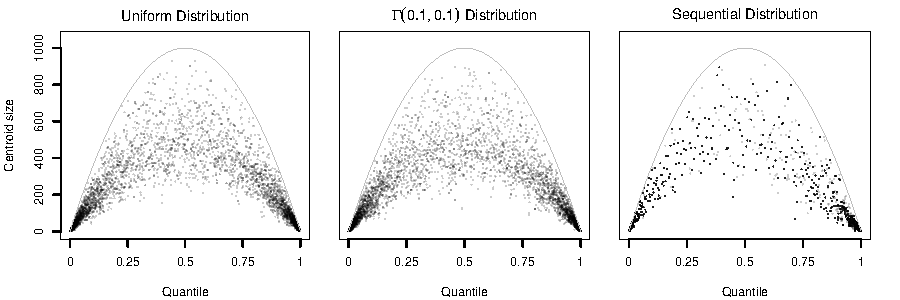
\includegraphics[width=6in]{sizes.pdf} 
   \caption{The $t$-digest algorithm respects the size limit for centroids.  The solid grey line indicates the size limit.  These diagrams also shows actual centroid weights for 5 test runs on $100,000$ samples from a uniform, $\Gamma(0.1, 0.1)$ and sequential uniform distribution.  In spite of the underlying distribution being skewed by roughly $30$ orders of magnitude of difference in probability density for the $\Gamma$ distribution, the centroid weight distribution is bounded and symmetric as intended.  For the sequential uniform case, values are produced in sequential order with three passes through the $[0,1]$ interval with no repeated values.  In spite of the lack of repeats, successive passes result in many centroids at the quantiles with the same sizes.  In spite of this, sequential presentation of data results in only a small asymmetry in the resulting size distribution and no violation of the intended size limit.}
   \label{fig:gamma-sizes}
\end{figure}

The key property of this algorithm is that the final list of centroids $C$ is very close to what would have been obtained by simply sorting and then grouping adjacent values in $X$ into groups with the desired size bounds.  Clearly, such groups could be used to compute all of the rank statistics of interest here and if there are bounds on the sizes of the groups, then we have comparable bounds on the accuracy of the rank statistics in question.

That this algorithm does produce such an approximation is more difficult to prove rigorously, but an empirical examination is enlightening.  Figure \ref{fig:deviation} shows the deviation of samples assigned to centroids for uniform and highly skewed distributions.  These deviations are normalized by the half the distance between the adjacent two centroids.
\begin{figure}[htb] %  figure placement: here, top, bottom, or page
   \centering
   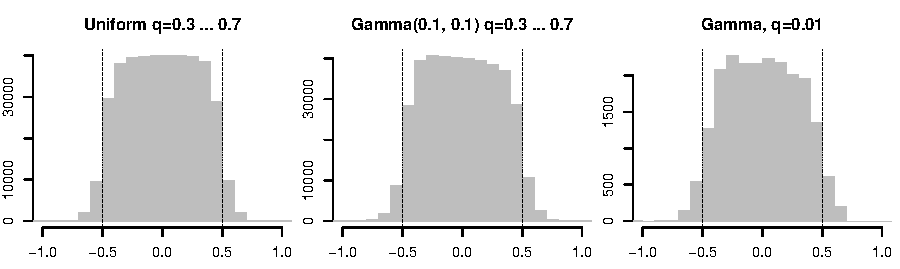
\includegraphics[width=6in]{deviation.pdf} 
   \caption{The deviation of samples assigned to a single centroid.  The horizontal axis is scaled to the distance to the adjacent centroid so a value of 0.5 is half-way between the two centroids. There are two significant observations to be had here.  The first is that relatively few points are assigned to a centroid that are beyond the midpoint to the next cluster.  This bears on the accuracy of this algorithm.  The second observation is that samples are distributed relatively uniformly between the boundaries of the cell.  This affects the interpolation method to be chosen when working with quantiles. The three graphs show, respectively, centroids from $q \in [0.3, 0.7]$ from a uniform distribution, centroids from the same range of a highly skewed $\Gamma(0.1, 0.1)$ and centroids from $q \in [0.01, 0.015]$ in a $\Gamma(0.1, 0.1)$ distribution.  This last range is in a region where skew on the order of $10^{22}$ is found. }
   \label{fig:deviation}
\end{figure}
This relatively uniform distribution for deviations among the samples assigned to a centroid is found for uniformly distributed samples as well as for extremely skewed data.  For instance, the $\Gamma(0.1, 0.1)$ distribution has a $0.01$ quantile of $6.07 \times 10^{-20}$, a median of $0.006$ and a mean of $1$.  This means that the distribution is very skewed.  In spite of this, samples assigned to centroids near the first percentile are not noticeably skewed within the centroid.  The impact of this uniform distribution is that linear interpolation allows accuracy considerably better than $q(1-q)/\delta$.

\subsection{Finding the cumulative distribution at a point}
Algorithm \ref{alg:quantile} shows how to compute the cumulative distribution $P(x)=\int_{-\infty}^x p(\alpha) \, d\alpha$ for a given value of $x$ by summing the contribution of uniform distributions centered at each the centroids.  Each of the centroids is assumed to extend symmetrically around the mean for half the distance to the adjacent centroid.

 \begin{algorithm}[b]
 \label{alg:quantile}
\SetKw{KwTo}{in}\SetKwFor{For}{for}{\string:}{}
\SetKwIF{If}{ElseIf}{Else}{if}{:}{elif}{else:}{}
\SetKwFor{While}{while}{:}{fintq}
\SetKwFor{For}{for}{\string:}{}
\SetNoFillComment
\KwIn{Centroids derived from distribution $p(x)$, $C = [ \ldots [m_i, s_i, k_i] \ldots ]$ , value $x$ }
\KwOut{Estimated value of $q = \int_{-\infty}^x p(\alpha) d \alpha$} 
$t = 0$, $N = \sum_i k_i$\;
\For {$i \in 1\ldots m$} {
    \uIf {$i < m$} {
      $\Delta \gets (c_{i+1}.\mathtt{mean} - c_i.\mathtt{mean})/2$\;
    } \Else {
      $\Delta \gets (c_{i}.\mathtt{mean} - c_{i-1}.\mathtt{mean})/2$\;
    }
    $z = \max(-1, (x-m_i)/\Delta)$\;
  \If {$z < 1$} {
    \Return $( \frac{t}{N} + \frac{k_i} N \frac{z+1} {2})$
  }
  $t \gets t + k_i$\;
}
\Return $1$
\caption{Estimate quantile $C.\mathtt{quantile}(x)$}
\end{algorithm}

For all centroids except one, this contribution will be either $0$ or $c_i.\mathtt{count}/N$ and the one centroid which straddles the desired value of $x$ will have a {\em pro rata} contribution somewhere between $0$ and $c_i.\mathtt{count}/N$. Moreover, since each centroid has count at most $\delta N$ the accuracy of $q$ should be accurate on a scale of $\delta$.  Typically, the accuracy will be even better due to the interpolation scheme used in the algorithm and because the largest centroids are only for values of $q$ near $0.5$.

The empirical justification for using a uniform distribution for each centroid can be seen by referring to again to Figure \ref{fig:deviation}.  

\subsection{Inverting the cumulative distribution}
Computing an approximation of the $q$ quantile of the data points seen so far can be done by ordering the centroids by ascending mean.  The running sum of the centroid counts will range from $0$ to $N=\sum c_i.\mathtt{count}$.  One particular centroid will have a count that straddles the desired quantile $q$ and interpolation can be used to estimate a value of $x$.  This is shown in Algorithm \ref{alg:estimate-quantile}.   Note that at the extreme ends of the distribution as observed, each centroid will represent a single sample so maximum resolution in $q$ will be retained.

 \begin{algorithm}[b]
 \label{alg:estimate-quantile}
\SetKw{KwTo}{in}\SetKwFor{For}{for}{\string:}{}
\SetKwIF{If}{ElseIf}{Else}{if}{:}{elif}{else:}{}
\SetKwFor{While}{while}{:}{fintq}
\SetKwFor{For}{for}{\string:}{}
\SetNoFillComment
\KwIn{Centroids derived from distribution $p(x)$, $C = [c_1 \ldots c_m ]$ , value $q$}
\KwOut{Estimated value $x$ such that $q = \int_{-\infty}^x p(\alpha) d \alpha$} 
$t = 0$, $q \gets q \sum c_i.\mathtt{count}$\;
\For {$i \in 1\ldots m$} {
  $k_i = c_i.\mathtt{count}$\;
  $m_i = c_i.\mathtt{mean}$\;
  \If {$q < t + k_i$} {
    \uIf {$i = 1$} {
      $\Delta \gets (c_{i+1}.\mathtt{mean} - c_i.\mathtt{mean})$\;
    } \uElseIf {$i = m$} {
      $\Delta \gets (c_{i}.\mathtt{mean} - c_{i-1}.\mathtt{mean})$\;
    } \Else {
      $\Delta \gets (c_{i+1}.\mathtt{mean} - c_{i-1}.\mathtt{mean})/2$\;
    }
    \Return $m_i + \left( \frac {q-t} {k_i} - \frac 1 2 \right) \Delta$
  } 
  $t \gets t + k_i$
}
\Return $ c_m.\mathtt{mean}$
\caption{Estimate value at given quantile $C.\mathtt{icdf}(q)$}
\end{algorithm}

\subsection{Computing the trimmed mean}
The trimmed mean of $X$ for the quantile range $Q = [q_0,q_1]$ can be computed by computing a weighted average of the means of centroids that have quantiles in $Q$.  For centroids at the edge of $Q$, a {\em pro rata} weight is used that is based on an interpolated estimate of the fraction of the centroid's samples that are in $Q$.  This method is shown as Algorithm \ref {alg:estimate-trimmed-mean}.

 \begin{algorithm}[b]
 \label{alg:estimate-trimmed-mean}
\SetKw{KwTo}{in}\SetKwFor{For}{for}{\string:}{}
\SetKwIF{If}{ElseIf}{Else}{if}{:}{elif}{else:}{}
\SetKwFor{While}{while}{:}{fintq}
\SetKwFor{For}{for}{\string:}{}
\SetNoFillComment
\KwIn{Centroids derived from distribution $p(x)$, $C = [ \ldots [m_i, s_i, k_i] \ldots ]$ , limit values $q_0, q_2$}
\KwOut{Estimate of mean of values $x \in [q_0, q_1]$} 
$s = 0$, $k = 0$\;
$t = 0$, $q_1 \gets q_1 \sum k_i$, $q_1 \gets q_1 \sum k_i$\;
\For {$i \in 1\ldots m$} {
  $k_i = c_i.\mathtt{count}$\;
  \uIf {$q_1 < t+k_i$} {
    \uIf {$i > 1$} {
      $\Delta \gets (c_{i+1}.\mathtt{mean} - c_{i-1}.\mathtt{mean})/2$\;
    } \uElseIf {$i < m$} {
      $\Delta \gets (c_{i+1}.\mathtt{mean} - c_i.\mathtt{mean})$\;
    } \Else {
      $\Delta \gets (c_{i}.\mathtt{mean} - c_{i-1}.\mathtt{mean})$\;
    }
    $\eta = \left( \frac {q-t} {k_i} - \frac 1 2 \right) \Delta$\;
    $s \gets s + \eta \,k_i \,c_i.\mathtt{mean}$\;
    $k \gets k + \eta \,k_i$\;
  } 
  \uIf {$q_2 < t+k_i$} {
    \uIf {$i > 1$} {
      $\Delta \gets (c_{i+1}.\mathtt{mean} - c_{i-1}.\mathtt{mean})/2$\;
    } \uElseIf {$i < m$} {
      $\Delta \gets (c_{i+1}.\mathtt{mean} - c_i.\mathtt{mean})$\;
    } \Else {
      $\Delta \gets (c_{i}.\mathtt{mean} - c_{i-1}.\mathtt{mean})$\;
    }
    $\eta = \left(\frac 1 2 - \frac {q-t} { k_i}  \right) \Delta$\;
    $s \gets s - \eta \,k_i \,c_i.\mathtt{mean}$\;
    $k \gets k - \eta \,k_i$\;
  } 
  $t \gets t + k_i$
}
\Return $s/k$
\caption{Estimate trimmed mean.  Note how centroids at the boundary are included on a {\em pro rata} basis.}
\end{algorithm}
\section{Empirical Assessment}
\subsection{Accuracy of estimation for uniform and skewed distributions}
Figure \ref{fig:uniform-error} shows the error levels achieved with $t$-digest in estimating quantiles of 100,000 samples from a uniform and from a skewed distribution.  In these experiments $\delta=0.01$ was used since it provides a good compromise between accuracy and space.  There is no visible difference in accuracy between the two underlying distributions in spite of the fact that the underlying densities differ by more roughly 30 orders of magnitude.  The accuracy shown here is computed by comparing the computed quantiles to the actual empirical quantiles for the sample used for testing and is shown in terms of $q$ rather than the underlying sample value.  At extreme values of $q$, the actual samples are preserved as centroids with weight $1$ so the observed for these extreme values is zero relative to the original data.  For the data shown here, at $q=0.001$, the maximum weight on a centroid is just above $4$ and centroids in this range have all possible weights from $1$ to $4$.  Errors are limited to, not surprisingly, just a few parts per million or less.  For more extreme quantiles, the centroids will have fewer samples and the results will typically be exact.
\begin{figure}[htb] %  figure placement: here, top, bottom, or page
   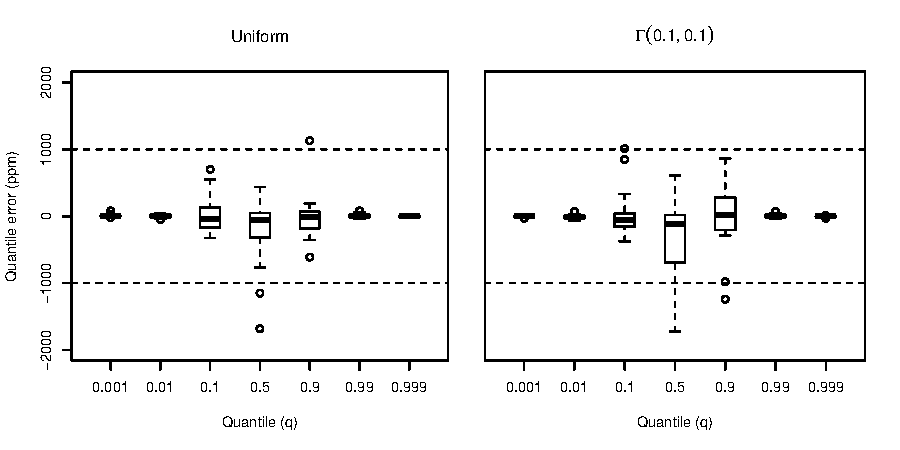
\includegraphics[width=6in]{error.pdf} 
   \caption{The absolute error of the estimate of the cumulative distribution function $q = \int_{-\infty}^x p(\alpha) \, d\alpha$ for the uniform and $\Gamma$ distribution for 5 runs, each with 100,000 data points.  As can be seen, the error is dramatically decreased for very high or very low quantiles (to a few parts per million).  The precision setting used here, $1/\delta = 100$, would result in uniform error of 10,000 ppm without adaptive bin sizing and interpolation.}
   \label{fig:uniform-error}
\end{figure}

Obviously, with the relatively small numbers of samples such as are used in these experiments, the accuracy of $t$-digests for estimating quantiles of the underlying distribution cannot be better than the accuracy of these estimates computed using the sample data points themselves.  For the experiments here, the errors due to sampling completely dominate the errors introduced by $t$-digests, especially at extreme values of $q$.  For much larger sample sets of billions of samples or more, this would be less true and the errors shown here would represent the accuracy of approximating the underlying distribution.

It should be noted that using a Q-Digest implemented with long integers is only able to store data with no more than 20 significant decimal figures.  The implementation in stream-lib only retains 48 bits of significants, allowing only about 16 significant figures.  This means that such a Q-digest would be inherently unable to even estimate the quantiles of the $\Gamma$ distribution tested here.

\subsection{Persisting $t$-digests}
For the accuracy setting and test data used in these experiments, the $t$-digest contained $820-860$ centroids.  The results of $t$-digest can thus be stored by storing this many centroid means and weights.  If centroids are kept as double precision floating point numbers and counts kept as 4-byte integers, the $t$-digest resulting from from the accuracy tests described here would require about 10 kilobytes of storage for any of the distributions tested.

This size can be substantially decreased, however.  One simple option is to store differences between centroid means and to use a variable byte encoding such as zig-zag encoding to store the cluster size.  The differences between successive means are at least three orders of magnitude smaller than the means themselves so using single precision floating point to store these differences can allow the $t$-digest from the tests described here to be stored in about $4.6$ kilobytes while still regaining nearly 10 significant figures of accuracy in the means.  This is roughly equivalent to the precision possible with a Q-digest operating on 32 bit integers, but the dynamic range of $t$-digests will be considerably higher and the accuracy is considerably better.

\subsection{Space/Accuracy Trade-off}
Not surprisingly, there is a strong trade-off between the size of the $t$-digest as controlled by the compression parameter $1/\delta$ and the accuracy which which quantiles are estimated.  Quantiles at $0.999$ and above or $0.001$ or below were estimated to within a small fraction of 1\% regardless of digest size.  Accurate estimates of the median require substantially larger digests.  Figure \ref{fig:accuracy-1} shows this basic trade-off.

\begin{figure}[htb] %  figure placement: here, top, bottom, or page
   \centering
   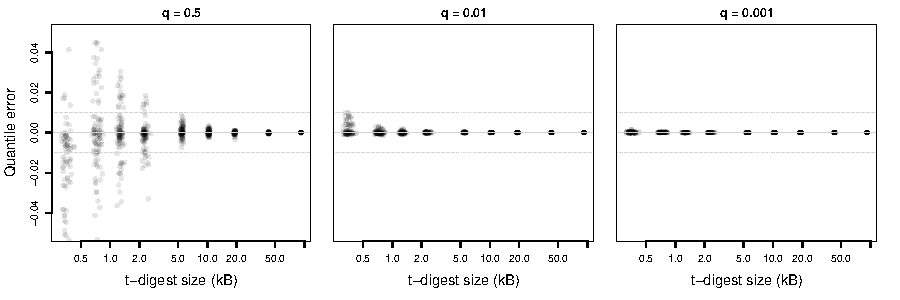
\includegraphics[width=6in]{error-scaling.pdf} 
   \caption{Accuracy is good for extreme quantiles regardless of digest size.  From left to right, these panels show accuracy of estimates for $q=0.5, 0.01$ and $0.001$ as a function the serialized size of the $t$-digest.  Due to symmetry, these are equivalent to accuracy for $q=0.5, 0.99$, and $0.999$ as well. For mid quantiles such as the median ($q=0.5$), moderate digest sizes of a few kilobytes suffice to get better than 1\% accuracy, but a digest must be 20kB or more to reliably achieve 0.1\% accuracy.  In contrast, accuracy for the $0.1\%$-ile (or $99.9\%$-ile) reaches a few parts per million for digests larger than about 5 kB.  Note that errors for $q=0.5$ and digests smaller than 1 kB are off the scale shown here at nearly 10\%.  All panels were computed using 100 runs with 100,000 samples.  Compression parameter ($1/\delta$) was varied from 2 to 1000 in order to vary the size of the resulting digest.  Sizes shown were encoded using 4 byte floating point delta encoding for the centroid means and variable byte length integer encoding.}
   \label{fig:accuracy-1}
\end{figure}
The size of the resulting digest depends strongly on the compression parameter $1/\delta$ as shown in the left panel of Figure \ref{fig:accuracy-2}.  Size of the digest also grows roughly with the log of the number of samples observed, at least in the range of 10,000 to 10,000,000 samples shown in the right panel of Figure \ref{fig:accuracy-2}.

\begin{figure}[htb] %  figure placement: here, top, bottom, or page
   \centering
   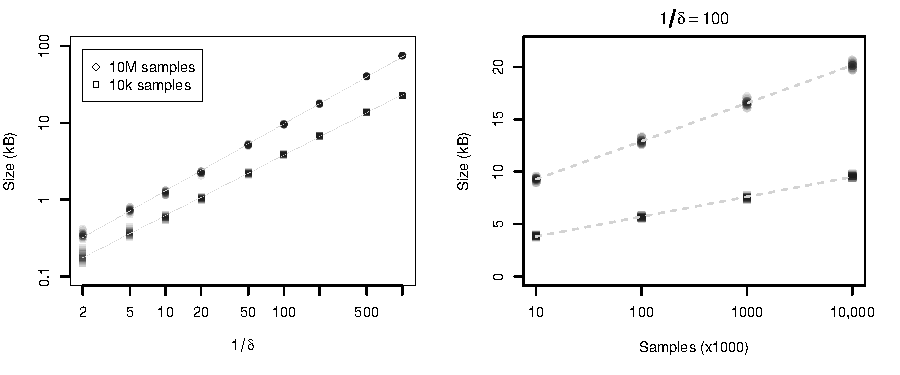
\includegraphics[width=6in]{scaling.pdf} 
   \caption{Size of the digest scales sub-linearly with compression parameter ($\alpha \approx 0.7 \ldots 0.9$) for fixed number of points.  Size scales approximately logarithmically with number of points for fixed compression parameter.  The panel on the right is for $1/\delta = 100$.  The dashed lines show best-fit log-linear models.  In addition, the right panel shows the memory size required for the GK01 algorithm if 6 specific quantiles are desired.}
   \label{fig:accuracy-2}
\end{figure}

\subsection{Computing $t$-digests in parallel}
With large scale computations, it is important to be able to compute aggregates like the $t$-digest on portions of the input and then combine those aggregates.  

For example, in a map-reduce framework such as Hadoop, a combiner function can compute the $t$-digest for the output of each mapper and a single reducer can be used to compute the $t$-digest for the entire data set.  

Another example can be found in certain databases such as Couchbase or Druid which maintain tree structured indices and allow the programmer to specify that particular aggregates of the data being stored can be kept at interior nodes of the index.  The benefit of this is that aggregation can be done almost instantaneously over any contiguous sub-range of the index.  The cost is quite modest with only a $O(\log(N))$ total increase in effort over keeping a running aggregate of all data.  In many practical cases, the tree can contain only two or three levels and still provide fast enough response.  For instance, if it is desired to be able to compute quantiles for any period up to years in 30 second increments, simply keeping higher level $t$-digests at the level of 30 seconds and days is likely to be satisfactory because at most about 10,000 digests are likely to need merging even for particularly odd intervals.  If almost all queries over intervals longer than a few weeks are day aligned, the number of digests that must be merged drops to a few thousand.
\begin{figure}[htb] %  figure placement: here, top, bottom, or page
   \centering
   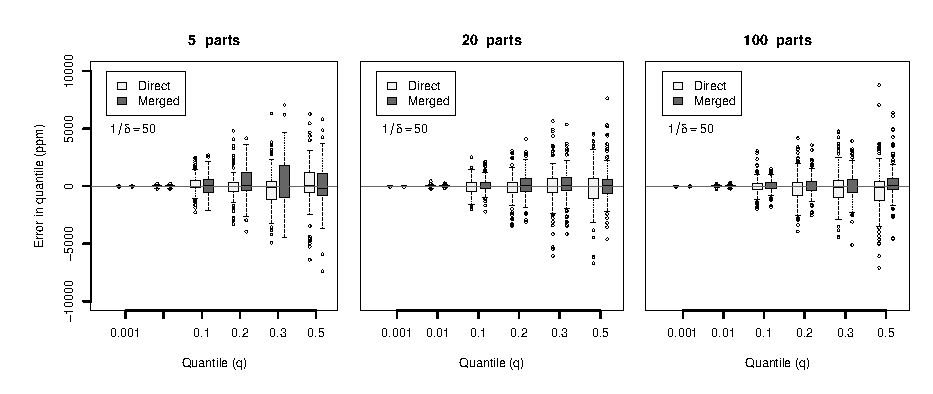
\includegraphics[width=6in]{merge.eps} 
   \caption{Accuracy of a $t$-digest accumulated directly is nearly the same as when the digest is computed by combining digests from 20 or 100 equal sized portions of the data.  Repeated runs of this test occasionally show the situation seen in the left panel where the accuracy for digests formed from 5 partial digests show slightly worse accuracy than the non-subdivided case.  This sub-aggregation property allows efficient use of the $t$digest in map-reduce and database applications.  Of particular interest is the fact that accuracy actually improves when the input data is broken in to many parts as is shown in the right hand panel.  All panels were computed by 40 repetitions of aggregating 100,000 values. Accuracy for directly accumulated digests is shown on the left of each pair with the white bar and the digest of digest accuracy is shown on the right of each pair by the dark gray bar.}
   \label{fig:merge}
\end{figure}

Merging $t$-digests can be done many ways.  The algorithm whose results are shown here consisted of simply making a list of all centroids from the $t$-digests being merged, shuffling that list, and then adding these centroids, preserving their weights, to a new $t$-digest.

\subsection{Comparison with Q-digest}
The prototype implementation of the $t$-digest completely dominates the implementation of the Q-digest from the popular stream-lib package \cite{github:stream} when size of the resulting digest is controlled.  This is shown in Figure \ref{fig:qd-comparison}.  In the left panel, the relationship between the effect of the compression parameter for Q-digest is compared to the similar parameter $1/\delta$ for the $t$-digest.  For the same value of compression parameter, the sizes of the two digests is always within a factor of 2 for practical uses.  The middle and right panel show accuracies for uniform and $\Gamma$ distributions.  
\begin{figure}[htb] %  figure placement: here, top, bottom, or page
   \centering
   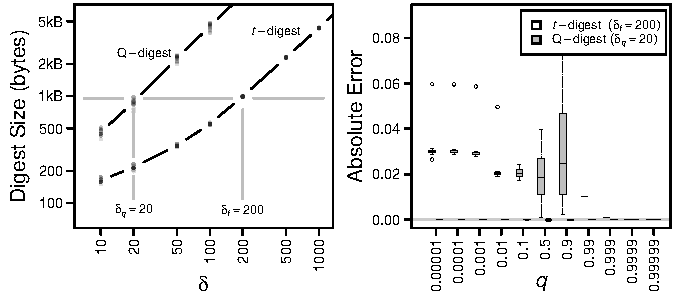
\includegraphics[width=6in]{qd-sizes.pdf} 
   \caption{The left panel shows the size of a serialized Q-digest versus the size of a serialized t-digest for various values of $1/\delta$ from 2 to 100,000.  The sizes for the two kinds of digest are within a factor of 2 for all compression levels.  The middle and right panels show the accuracy for a particular setting of $1/\delta$ for Q-digest and t-digest.  For each quantile, the Q-digest accuracy is shown as the left bar in a pair and the t-digest accuracy is shown as the right bar in a pair.  Note that the vertical scale in these diagrams are one or two orders of magnitude larger than in the previous accuracy graphs and that in all cases, the accuracy of the t-digest is dramatically better than that of the Q-digest even though the serialized size of the each is within 10\% of the other.   Note that the errors in the right hand panel are systematic quantization errors introduced by the use of integers in the Q-digest algorithm.  Any distribution with very large dynamic range will show the same problems.}
   \label{fig:qd-comparison}
\end{figure}

As expected, the $t$-digest has very good accuracy for extreme quantiles while the Q-digest has constant error across the range.  Interestingly, the accuracy of the Q-digest is at best roughly an order of magnitude worse than the accuracy of the $t$-digest even.  At worse, with extreme values of $q$, accuracy is several orders of magnitude worse.  This situation is even worse with a highly skewed distribution such as with the $\Gamma(0.1, 0.1)$ shown in the right panel.  Here, the very high dynamic range introduces severe quantization errors into the results.  This quantization is inherent in the use of integers in the Q-digest.

For higher compression parameter values, the size of the Q-digest becomes up to two times smaller than the $t$-digest, but no improvement in the error rates is observed.

\subsection{Speed}
The current implementation has been primarily optimized for ease of development, not execution speed.  As it is, running on a single core of a 2.3 GHz Intel Core i5, it typically takes 2-3 microseconds to process each point after JIT optimization has come into effect.  It is to be expected that a substantial improvement in speed could be had by profiling and cleaning up the prototype code.

\section{Conclusion}
The $t$-digest is a novel algorithm that dominates the previously state-of-the-art Q-digest in terms of accuracy and size.  The $t$-digest provides accurate on-line estimates of a variety of of rank-based statistics including quantiles and trimmed mean.  The algorithm is simple and empirically demonstrated to exhibit accuracy as predicted on theoretical grounds.  It is also suitable for parallel applications.  Moreover, the $t$-digest algorithm is inherently on-line while the Q-digest is an on-line adaptation of an off-line algorithm.

The $t$-digest algorithm is available in the form of an open source, well-tested implementation from the author.  It has already been adopted by the Apache Mahout and stream-lib projects and is likely to be adopted by other projects as well.

%\subsection{}
\bibliographystyle{alpha}
\bibliography{refs}{}

\end{document}  
